\documentclass{ctexart}
\usepackage{xcolor}
\usepackage{setspace}
\usepackage{tikz}
\usepackage{ctex}
\usepackage{geometry}
\usepackage{amsmath}
\usepackage{graphicx} 
\usepackage{subfigure}
\usepackage{float}
\usepackage{algorithm}  
\usepackage{algorithmicx}  
\usepackage{algpseudocode} 
\usepackage{url}
\usepackage{amsthm, amssymb, appendix, bm, graphicx, hyperref, mathrsfs}
\usepackage{tabularx}
\usepackage{booktabs} %需要加载宏包{booktabs}
\usepackage{multirow}
\usepackage{diagbox} % 加载宏包
\usepackage{pifont}

\usepackage{siunitx}
\usepackage{listings}
\usepackage{float}
\pagestyle{plain}

\usetikzlibrary{datavisualization}
\usetikzlibrary{arrows,shapes,chains}
\usepackage{listings}
\lstset{language=C++}
\lstset{breaklines}
\lstset{extendedchars=false}
\lstset{numbers=left}
\geometry{a4paper,left=2.5cm,right=2.5cm,top=2.5cm,bottom=2.5cm}
\CTEXsetup[format={\Large\bfseries\centering}]{section}
\tikzstyle{startstop} = [rectangle,rounded corners, minimum width=3cm,minimum height=1cm,text centered, text width=6cm,draw=black]
\tikzstyle{io} = [trapezium, trapezium left angle = 70,trapezium right angle=110,minimum width=5cm,minimum height=1cm,text centered,draw=black,fill=white]
\tikzstyle{process} = [rectangle,minimum width=3cm,minimum height=1cm,text centered,text width =3cm,text width=6cm,draw=black]
\tikzstyle{decision} = [diamond,minimum width=3cm,minimum height=1cm,text centered,text width=6cm,aspect=2,draw=black,thin]
\tikzstyle{arrow} = [thick,->,>=stealth]
\renewcommand{\algorithmicrequire}{\textbf{Input:}}  % Use Input in the format of Algorithm  
\renewcommand{\algorithmicensure}{\textbf{Output:}} % Use Output in the format of Algorithm  
\newcommand{\subsubsubsection}[1]{\paragraph{#1}\mbox{}\\}
\setcounter{secnumdepth}{4} % how many sectioning levels to assign numbers to
\setcounter{tocdepth}{4} % how many sectioning levels to show in ToC
\begin{document}
\begin{spacing}{2.0}
    \begin{center}
        {\LARGE\textbf{基于xx的xx的研究}}\\
        {\Large\textbf{摘要}}\\
    \end{center}
\end{spacing}

本文研究的是xx,通过建立xx模型和xx模型,求解得到xx,获得xx。

首先采用xx对已知数据进行(插值补全),为模型建立提供数据基础。

\textbf{针对问题一:}\quad 本文对xx建立了xx模型,描述...(针对...)【重要模型和重要结果加粗处理】

\textbf{针对问题二:}\quad 建立模型+模型参数设置+方法阐述(中间过程结果可适当分析)+所得结果(展示所有要求结果,可不进行分析)

\textbf{针对问题三:}\quad 本题需要xxx(做什么)。按做法步骤,关键部分展示,最后写出数据结果

\textbf{针对问题四:}\quad 本题提出xx,在问题x的基础上,...。【每个部分用一句话概括】


\quad

\textbf{关键词: \quad 重要研究对象\quad 主要模型\quad 主要求解方法 }

\newpage
\section{问题的背景与重述}
\subsection{问题的背景}
研究意义和研究进展

因此探究xx问题具有重要的研究价值。

\subsection{问题的重述}

根据xx观察数据,解决下列问题:

(1)用一两句话改写题目内容:主要包括需要完成什么任务

(2)

(3)

(4)

\section{问题分析}
对于问题一:问题解决的思路展现(讨论时确定的框架-会议记录)

对于问题二:不需要呈现结果

对于问题三:或可增加基于xx数据图,我们可以发现...,因而采用...(选择理由可简单阐述)

对于问题四:

\section{模型假设}
1. \quad 假设(题中假设)

2. \quad 假设所给数据均真实可靠

3. \quad 做题过程中的前提假设
\section{符号说明}

\begin{table}[!htbp]
    \centering
    \begin{tabular}{ccc}
    \toprule
    符号& 含义& 单位\\
    \midrule
    $S_i(x)$&第i段x的三次样条插值函数&/\\
    x(T)&温度为T时的乙醇转化率&\%\\
    \bottomrule
    \end{tabular}
    %\caption{这是一张三线表}\label{tab:aStrangeTable}  标题放在这里也是可以的
    \end{table}

\section{数据预处理}
首先我们对附件x中的数据进行观察分析,发现xx(低质量数据问题),这些都给后续的分析带来不便,因此我们用xx,令xx,(对其中的数据进行插值补全)。

处理方法简述

处理后的数据结果展示(图/表)

在(表一)中,xxx,(增加了数据点数量),可以有效地提高问题中模型拟合的准确性。
\section{模型的建立与求解}

注:模型建立在做完后有足够时间考虑加分项-改进经典模型,创新性;同一问题使用两个或以上合理模型进行求解,需做对比和评价

模型求解-包含算法设计与选择(原理、思想、依据、采用软件理由及名称等),算法步骤(对求解无帮助的计算过程和中间结果不需列出),算法实现;另:1.命题叙述符合数学命题$\quad$ 2.要求回答的问题(数值结果,结论)逐项解答,结论明确$\quad$ 3.列出多组数据进行比较、分析 $\quad$ 4.运用流程图、模式图、数据表灵活展示结果

模型检验-包括结果正确性的分析、检验,模型合理性的分析、检验
\subsection{问题一模型的建立与求解}
\subsubsection{数据可视化}
为了更加直观方便地分析xx与xx之间的关系,我们考虑对xx数据进行可视化,画出xx如下:

方程拟合与结论分析

注:重点给出从数据中获取的信息,为建模作铺垫

\subsubsection{(第一小问)}
将一个大问转化成几个小问,按顺序阐述
\subsubsubsection{模型的建立}
通过图/题目信息获取信息,给出对应模型,需要说明模型思考的来源

对于较复杂问题,可以采用:

\textbf{Step1 $\quad$}

\textbf{Step2 $\quad$}

\textbf{Step3 $\quad$}

\subsubsubsection{结果及分析}
算法求解、数据展示、数据分析、结果展示、结果分析,不符合预期的异常值分析,得出最终结论

数据结果或表太长可以加在附录当中

\subsubsection{(第二小问)}
\subsubsubsection{模型的建立}
\subsubsubsection{结果及分析}
\subsubsection{(补充内容)}
展示优势的部分,加上思考延伸的内容,如:缺失值的预测等

\subsection{问题二模型的建立与求解}
\subsubsection{xx模型的建立}
模型的相关阐释,并解释为什么用这种模型(概览)

【三线表】

\begin{table}[!htbp]
\centering
\caption{这是一张三线表}\label{tab:aStrangeTable}%添加标题 设置标签
\begin{tabular}{ccc}
\toprule
姓名& 学号& 性别\\
\midrule
Steve Jobs& 001& Male\\
Bill Gates& 002& Female\\
\bottomrule
\end{tabular}
%\caption{这是一张三线表}\label{tab:aStrangeTable}  标题放在这里也是可以的
\end{table}

以上:{table}有若干可选参数 [!htbp]

h代表here,将表格排在当前文字位置

t 表示将表格放在下一页的 top (页首)

b 表示将表格放在当前页的 bottom (底部)

!表示忽略美观因素,尽可能按照参数指定的方式来处理表格浮动位置。

表格将会按照所给参数,依次尝试按照每个参数进行排版,当无法排版时,将会按照下一个参数

【单元格合并】

\begin{table}[!htbp]
\centering
\begin{tabular}{|c|c|c|c|c|c|c|}
\hline

\multicolumn{2}{|c|}{ \multirow{2}*{$S_i$} }& \multicolumn{4}{c|}{事件} &\multirow{2}*{max}\\
\cline{3-6}
\multicolumn{2}{|c|}{}&50&100&150&200&\\
\hline
\multirow{4}*{策略}&50&0&100&200&300&300\\
\cline{2-7}
&100&100&0&100&200&200\\
\cline{2-7}
&150&200&100&0&100&200\\
\cline{2-7}
&200&300&200&100&0&300\\
\hline
\end{tabular}
\end{table}

【斜线表头】

\begin{table}[!htbp]
\centering
\begin{tabular}{|c|c|c|c|}
\hline
\diagbox{甲}{$\alpha_{i,j}$}{乙}&$\beta_1$&$\beta_2$&$\beta_3$\\ %添加斜线表头
\hline
$\alpha_1$&-4&0&-8\\
\hline
$\alpha_2$&3&2&4\\
\hline
$\alpha_3$&16&1&-9\\
\hline
$\alpha_4$&-1&1&7\\
\hline
\end{tabular}
\end{table}

【混合类型】

需要添加参数$\backslash$ diagbox[innerwidth=2cm](参数大小取决于列宽度)解决

\begin{table}[!htbp]
  \centering
  \begin{tabular}{|c|c|c|c|c|c|c|}
   \hline
   \multicolumn{2}{|c|}{\multirow{2}*{\diagbox[innerwidth=2cm]{$S_i$}{$\lambda_i$}}}& \multicolumn{4}{c|}{事件} &\multirow{2}*{max}\\
   \cline{3-6}
   \multicolumn{2}{|c|}{}&50&100&150&200&\\
   \hline
   \multirow{4}*{策略}&50&0&100&200&300&300\\
   \cline{2-7}
   &100&100&0&100&200&200\\
   \cline{2-7}
   &150&200&100&0&100&200\\
   \cline{2-7}
   &200&300&200&100&0&300\\
   \hline
  \end{tabular}
 \end{table}











注:若模型阐释有许多前提假设,设立条件,可以一步步细化:

a.

b.

c.构建模型

公式表达方式【大括号】

\begin{equation}
		h_0(x)= \left\{
			      \begin{array}{ll}
					(1+2\frac{x-x_0}{x_1-x_0})(\frac{x-x_1}{x_0-x_1})^2 \quad x_0\le x\le x_1\\
					0 \quad x_1 < x\le x_n
				  \end{array}
		        \right.
\end{equation}
  






\begin{equation}
F^{HLLC}=\left\{
\begin{array}{rcl}
F_L       &      & {0      <      S_L}\\
F^*_L     &      & {S_L \leq 0 < S_M}\\
F^*_R     &      & {S_M \leq 0 < S_R}\\
F_R       &      & {S_R \leq 0}
\end{array} \right. 
\end{equation}


\subsubsection{模型的求解}
若可以借助工具直接解出,可以在这部分证明用这个工具的前提条件是否成立

\subsubsection{模型的结果与分析}
若利用工具,如SPSS,需解释各数据的实际意义,再得出结论

尽可能展示每一步求解的方法与结果,并分别给出结论,最后整合(可以结合第一问中得出的结论,使文章一脉相承)

\subsection{问题三模型的建立与求解}

本题的目标+总体思路

\subsubsection{xx的(拟合)模型}
\textbf{Step1 \quad }

\textbf{Step2 \quad }
\subsubsection{xx的(优化)模型}
利用xx,我们可以建立xx(单目标规划模型),来获得...

1)\textbf{决策变量:} 解释+具体符号/公式

2)\textbf{目标函数:}

3)\textbf{约束条件:}

\ding{172} xx约束:

\begin{equation}
    33 \le x_1 \le 200
\end{equation}

\ding{173} xx约束:

\begin{equation}
    33 \le x_2 \le 200
\end{equation}

综上所述,对xx建立优化模型如下:

\[
    max \quad y=1.1x_1+1.2x_2
\]
\begin{equation}
    s.t. \left\{
			      \begin{array}{ll}
                    33 \le x_1 \le 200\\
                    33 \le x_2 \le 200
				  \end{array}
		        \right.
\end{equation}

\subsubsection{结果的对比分析}

插入表/图

对数字结果进行分析(由上表数据...)

\subsubsection{结果的检验}
根据上表数据,可以发现...

与xx结论相符,从侧面验证了我们结论的正确性。

\subsection{问题四的分析解决}

注:一般为开放性问题,可以将思考得到的方面作为不同步分展开阐述。

需写出思考来源,如由上文结论,数据分析,文献资料,附件数据等

需加上扩展该部分内容的价值(现实意义等)










\section{模型的评价与推广}
\subsection{模型的优点}
1、着力讲文章的创新点与优势,例如:补全数据点增加准确性...

2、本文做了大量的图表来统计分析数据特点,更加直观地...

3、...

\subsection{模型的缺点}

1、结合模型假设对模型缺点点评,每个缺点写完后可以加改进措施/想法。

2、...

\subsection{灵敏度分析}

对数据提出的假设做分析,最好结合实际说明为什么可能出现这种情况,对应现实中的结果会如何改变。

不同的模型灵敏度分析的方面不同,共分为决策型模型(优化),动态模型,概率模型,线性回归/时间序列,涉及这些方面时需做相关探究。

\subsection{模型的推广}

本文主要建立的xx模型有哪些优点,有什么价值,适宜推广到哪些领域。以及本文所建立的xx模型有哪些优点,适合推广到xx等相关问题/研究工作中去。

\begin{thebibliography}{100}%此处数字为最多可添加的参考文献数量
    \bibitem{article1} 陈立辉,苏伟,蔡川  \emph{基于latex的web数学公式提取方法研究}[J],计算机科学,2017(06)
    \bibitem{article2} xx
    \bibitem{book1}William H ,Press,Saul A ,Teukolsky,William T ,VeterLing ,Brian P.Flannery,\emph{Numerical Recipes 3rd Edition:The Art of Scientific Computing }Cambridge University Press ,New York,2007    
\end{thebibliography}
\newpage
\begin{flushleft}
    \Large{ \textbf{附录}}

    ~\\

    \normalsize \textbf{附录说明:}

    1.xx图

    2.xx表

    3.xx程序

    4.xx程序

    5.xx程序

    6.xx程序

    ~\\

    附录1

    \begin{center}
        \begin{figure}[H]
            \begin{center}
                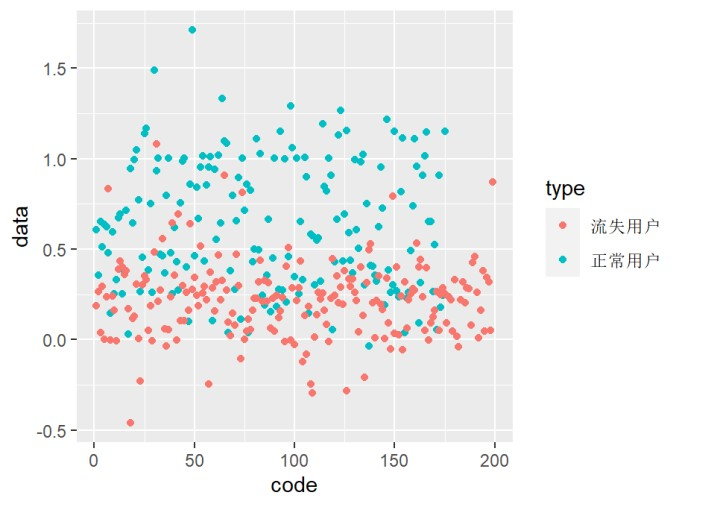
\includegraphics[width=1.00\linewidth]{pic/样图.jpg}
            \end{center}
        \end{figure}
    \end{center}

    附录2
    
    ~\\

    \begin{tabularx}{\textwidth}{|c|X|X|X|X|X|}
        \hline
        数字 &1&2&3&4&5\\
        \hline 
        字母 &A&B&C&D&E\\
        \hline 
        天干 & 甲 & 乙 & 丙 & 丁 & 戊 \\
        \hline
    \end{tabularx}

    ~\\

    附录3

    本部分代码使用的软件是Python

\definecolor{mygreen}{rgb}{0,0.6,0}  
\definecolor{mygray}{rgb}{0.5,0.5,0.5}  
\definecolor{mymauve}{rgb}{0.58,0,0.82}  
  
\lstset{ %  
  backgroundcolor=\color{white},   % choose the background color; you must add \usepackage{color} or \usepackage{xcolor}  
  basicstyle=\footnotesize,        % the size of the fonts that are used for the code  
  breakatwhitespace=false,         % sets if automatic breaks should only happen at whitespace  
  breaklines=true,                 % sets automatic line breaking  
  captionpos=bl,                    % sets the caption-position to bottom  
  commentstyle=\color{mygreen},    % comment style  
  deletekeywords={...},            % if you want to delete keywords from the given language  
  escapeinside={\%*}{*)},          % if you want to add LaTeX within your code  
  extendedchars=true,              % lets you use non-ASCII characters; for 8-bits encodings only, does not work with UTF-8  
  frame=single,                    % adds a frame around the code  
  keepspaces=true,                 % keeps spaces in text, useful for keeping indentation of code (possibly needs columns=flexible)  
  keywordstyle=\color{blue},       % keyword style  
  %language=Python,                 % the language of the code  
  morekeywords={*,...},            % if you want to add more keywords to the set  
  numbers=left,                    % where to put the line-numbers; possible values are (none, left, right)  
  numbersep=5pt,                   % how far the line-numbers are from the code  
  numberstyle=\tiny\color{mygray}, % the style that is used for the line-numbers  
  rulecolor=\color{black},         % if not set, the frame-color may be changed on line-breaks within not-black text (e.g. comments (green here))  
  showspaces=false,                % show spaces everywhere adding particular underscores; it overrides 'showstringspaces'  
  showstringspaces=false,          % underline spaces within strings only  
  showtabs=false,                  % show tabs within strings adding particular underscores  
  stepnumber=1,                    % the step between two line-numbers. If it's 1, each line will be numbered  
  stringstyle=\color{orange},     % string literal style  
  tabsize=2,                       % sets default tabsize to 2 spaces  
  %title=myPython.py                   % show the filename of files included with \lstinputlisting; also try caption instead of title  
}  
~\\
\lstinputlisting[language=Python]{decision_tree code.py}  

~\\

附录4

本部分代码使用的软件是Matlab

~\\

\lstinputlisting[language=Matlab]{A2.m}

~\\

附录5

本部分代码使用的软件是C++

~\\

\lstinputlisting[language=C++]{calc_p.cpp}

~\\

附录6

本部分代码使用的软件是R

~\\

\lstinputlisting[language=R]{可视化.R}

~\\


\end{flushleft}
\end{document}